%% bare_conf.tex
%% V1.4b
%% 2015/08/26
%% by Michael Shell
%% See:
%% http://www.michaelshell.org/
%% for current contact information.
%%
%% This is a skeleton file demonstrating the use of IEEEtran.cls
%% (requires IEEEtran.cls version 1.8b or later) with an IEEE
%% conference paper.
%%
%% Support sites:
%% http://www.michaelshell.org/tex/ieeetran/
%% http://www.ctan.org/pkg/ieeetran
%% and
%% http://www.ieee.org/

%%*************************************************************************
%% Legal Notice:
%% This code is offered as-is without any warranty either expressed or
%% implied; without even the implied warranty of MERCHANTABILITY or
%% FITNESS FOR A PARTICULAR PURPOSE! 
%% User assumes all risk.
%% In no event shall the IEEE or any contributor to this code be liable for
%% any damages or losses, including, but not limited to, incidental,
%% consequential, or any other damages, resulting from the use or misuse
%% of any information contained here.
%%
%% All comments are the opinions of their respective authors and are not
%% necessarily endorsed by the IEEE.
%%
%% This work is distributed under the LaTeX Project Public License (LPPL)
%% ( http://www.latex-project.org/ ) version 1.3, and may be freely used,
%% distributed and modified. A copy of the LPPL, version 1.3, is included
%% in the base LaTeX documentation of all distributions of LaTeX released
%% 2003/12/01 or later.
%% Retain all contribution notices and credits.
%% ** Modified files should be clearly indicated as such, including  **
%% ** renaming them and changing author support contact information. **
%%*************************************************************************


% *** Authors should verify (and, if needed, correct) their LaTeX system  ***
% *** with the testflow diagnostic prior to trusting their LaTeX platform ***
% *** with production work. The IEEE's font choices and paper sizes can   ***
% *** trigger bugs that do not appear when using other class files.       ***                          ***
% The testflow support page is at:
% http://www.michaelshell.org/tex/testflow/





\documentclass[conference]{IEEEtran}
% Some Computer Society conferences also require the compsoc mode option,
% but others use the standard conference format.
%
% If IEEEtran.cls has not been installed into the LaTeX system files,
% manually specify the path to it like:
% \documentclass[conference]{../sty/IEEEtran}





% Some very useful LaTeX packages include:
% (uncomment the ones you want to load)


% *** MISC UTILITY PACKAGES ***
%
%\usepackage{ifpdf}
% Heiko Oberdiek's ifpdf.sty is very useful if you need conditional
% compilation based on whether the output is pdf or dvi.
% usage:
% \ifpdf
%   % pdf code
% \else
%   % dvi code
% \fi
% The latest version of ifpdf.sty can be obtained from:
% http://www.ctan.org/pkg/ifpdf
% Also, note that IEEEtran.cls V1.7 and later provides a builtin
% \ifCLASSINFOpdf conditional that works the same way.
% When switching from latex to pdflatex and vice-versa, the compiler may
% have to be run twice to clear warning/error messages.






% *** CITATION PACKAGES ***
%
%\usepackage{cite}
% cite.sty was written by Donald Arseneau
% V1.6 and later of IEEEtran pre-defines the format of the cite.sty package
% \cite{} output to follow that of the IEEE. Loading the cite package will
% result in citation numbers being automatically sorted and properly
% "compressed/ranged". e.g., [1], [9], [2], [7], [5], [6] without using
% cite.sty will become [1], [2], [5]--[7], [9] using cite.sty. cite.sty's
% \cite will automatically add leading space, if needed. Use cite.sty's
% noadjust option (cite.sty V3.8 and later) if you want to turn this off
% such as if a citation ever needs to be enclosed in parenthesis.
% cite.sty is already installed on most LaTeX systems. Be sure and use
% version 5.0 (2009-03-20) and later if using hyperref.sty.
% The latest version can be obtained at:
% http://www.ctan.org/pkg/cite
% The documentation is contained in the cite.sty file itself.






% *** GRAPHICS RELATED PACKAGES ***
%
\ifCLASSINFOpdf
  % \usepackage[pdftex]{graphicx}
  % declare the path(s) where your graphic files are
  % \graphicspath{{../pdf/}{../jpeg/}}
  % and their extensions so you won't have to specify these with
  % every instance of \includegraphics
  % \DeclareGraphicsExtensions{.pdf,.jpeg,.png}
\else
  % or other class option (dvipsone, dvipdf, if not using dvips). graphicx
  % will default to the driver specified in the system graphics.cfg if no
  % driver is specified.
  % \usepackage[dvips]{graphicx}
  % declare the path(s) where your graphic files are
  % \graphicspath{{../eps/}}
  % and their extensions so you won't have to specify these with
  % every instance of \includegraphics
  % \DeclareGraphicsExtensions{.eps}
\fi
% graphicx was written by David Carlisle and Sebastian Rahtz. It is
% required if you want graphics, photos, etc. graphicx.sty is already
% installed on most LaTeX systems. The latest version and documentation
% can be obtained at: 
% http://www.ctan.org/pkg/graphicx
% Another good source of documentation is "Using Imported Graphics in
% LaTeX2e" by Keith Reckdahl which can be found at:
% http://www.ctan.org/pkg/epslatex
%
% latex, and pdflatex in dvi mode, support graphics in encapsulated
% postscript (.eps) format. pdflatex in pdf mode supports graphics
% in .pdf, .jpeg, .png and .mps (metapost) formats. Users should ensure
% that all non-photo figures use a vector format (.eps, .pdf, .mps) and
% not a bitmapped formats (.jpeg, .png). The IEEE frowns on bitmapped formats
% which can result in "jaggedy"/blurry rendering of lines and letters as
% well as large increases in file sizes.
%
% You can find documentation about the pdfTeX application at:
% http://www.tug.org/applications/pdftex





% *** MATH PACKAGES ***
%
%\usepackage{amsmath}
% A popular package from the American Mathematical Society that provides
% many useful and powerful commands for dealing with mathematics.
%
% Note that the amsmath package sets \interdisplaylinepenalty to 10000
% thus preventing page breaks from occurring within multiline equations. Use:
%\interdisplaylinepenalty=2500
% after loading amsmath to restore such page breaks as IEEEtran.cls normally
% does. amsmath.sty is already installed on most LaTeX systems. The latest
% version and documentation can be obtained at:
% http://www.ctan.org/pkg/amsmath





% *** SPECIALIZED LIST PACKAGES ***
%
%\usepackage{algorithmic}
% algorithmic.sty was written by Peter Williams and Rogerio Brito.
% This package provides an algorithmic environment fo describing algorithms.
% You can use the algorithmic environment in-text or within a figure
% environment to provide for a floating algorithm. Do NOT use the algorithm
% floating environment provided by algorithm.sty (by the same authors) or
% algorithm2e.sty (by Christophe Fiorio) as the IEEE does not use dedicated
% algorithm float types and packages that provide these will not provide
% correct IEEE style captions. The latest version and documentation of
% algorithmic.sty can be obtained at:
% http://www.ctan.org/pkg/algorithms
% Also of interest may be the (relatively newer and more customizable)
% algorithmicx.sty package by Szasz Janos:
% http://www.ctan.org/pkg/algorithmicx




% *** ALIGNMENT PACKAGES ***
%
%\usepackage{array}
% Frank Mittelbach's and David Carlisle's array.sty patches and improves
% the standard LaTeX2e array and tabular environments to provide better
% appearance and additional user controls. As the default LaTeX2e table
% generation code is lacking to the point of almost being broken with
% respect to the quality of the end results, all users are strongly
% advised to use an enhanced (at the very least that provided by array.sty)
% set of table tools. array.sty is already installed on most systems. The
% latest version and documentation can be obtained at:
% http://www.ctan.org/pkg/array


% IEEEtran contains the IEEEeqnarray family of commands that can be used to
% generate multiline equations as well as matrices, tables, etc., of high
% quality.




% *** SUBFIGURE PACKAGES ***
%\ifCLASSOPTIONcompsoc
%  \usepackage[caption=false,font=normalsize,labelfont=sf,textfont=sf]{subfig}
%\else
%  \usepackage[caption=false,font=footnotesize]{subfig}
%\fi
% subfig.sty, written by Steven Douglas Cochran, is the modern replacement
% for subfigure.sty, the latter of which is no longer maintained and is
% incompatible with some LaTeX packages including fixltx2e. However,
% subfig.sty requires and automatically loads Axel Sommerfeldt's caption.sty
% which will override IEEEtran.cls' handling of captions and this will result
% in non-IEEE style figure/table captions. To prevent this problem, be sure
% and invoke subfig.sty's "caption=false" package option (available since
% subfig.sty version 1.3, 2005/06/28) as this is will preserve IEEEtran.cls
% handling of captions.
% Note that the Computer Society format requires a larger sans serif font
% than the serif footnote size font used in traditional IEEE formatting
% and thus the need to invoke different subfig.sty package options depending
% on whether compsoc mode has been enabled.
%
% The latest version and documentation of subfig.sty can be obtained at:
% http://www.ctan.org/pkg/subfig




% *** FLOAT PACKAGES ***
%
%\usepackage{fixltx2e}
% fixltx2e, the successor to the earlier fix2col.sty, was written by
% Frank Mittelbach and David Carlisle. This package corrects a few problems
% in the LaTeX2e kernel, the most notable of which is that in current
% LaTeX2e releases, the ordering of single and double column floats is not
% guaranteed to be preserved. Thus, an unpatched LaTeX2e can allow a
% single column figure to be placed prior to an earlier double column
% figure.
% Be aware that LaTeX2e kernels dated 2015 and later have fixltx2e.sty's
% corrections already built into the system in which case a warning will
% be issued if an attempt is made to load fixltx2e.sty as it is no longer
% needed.
% The latest version and documentation can be found at:
% http://www.ctan.org/pkg/fixltx2e


%\usepackage{stfloats}
% stfloats.sty was written by Sigitas Tolusis. This package gives LaTeX2e
% the ability to do double column floats at the bottom of the page as well
% as the top. (e.g., "\begin{figure*}[!b]" is not normally possible in
% LaTeX2e). It also provides a command:
%\fnbelowfloat
% to enable the placement of footnotes below bottom floats (the standard
% LaTeX2e kernel puts them above bottom floats). This is an invasive package
% which rewrites many portions of the LaTeX2e float routines. It may not work
% with other packages that modify the LaTeX2e float routines. The latest
% version and documentation can be obtained at:
% http://www.ctan.org/pkg/stfloats
% Do not use the stfloats baselinefloat ability as the IEEE does not allow
% \baselineskip to stretch. Authors submitting work to the IEEE should note
% that the IEEE rarely uses double column equations and that authors should try
% to avoid such use. Do not be tempted to use the cuted.sty or midfloat.sty
% packages (also by Sigitas Tolusis) as the IEEE does not format its papers in
% such ways.
% Do not attempt to use stfloats with fixltx2e as they are incompatible.
% Instead, use Morten Hogholm'a dblfloatfix which combines the features
% of both fixltx2e and stfloats:
%
% \usepackage{dblfloatfix}
% The latest version can be found at:
% http://www.ctan.org/pkg/dblfloatfix




% *** PDF, URL AND HYPERLINK PACKAGES ***
%
%\usepackage{url}
% url.sty was written by Donald Arseneau. It provides better support for
% handling and breaking URLs. url.sty is already installed on most LaTeX
% systems. The latest version and documentation can be obtained at:
% http://www.ctan.org/pkg/url
% Basically, \url{my_url_here}.




% *** Do not adjust lengths that control margins, column widths, etc. ***
% *** Do not use packages that alter fonts (such as pslatex).         ***
% There should be no need to do such things with IEEEtran.cls V1.6 and later.
% (Unless specifically asked to do so by the journal or conference you plan
% to submit to, of course. )


% correct bad hyphenation here
\hyphenation{op-tical net-works semi-conduc-tor}

\usepackage{graphicx}
\graphicspath{ {./images/} }


\begin{document}
%
% paper title
% Titles are generally capitalized except for words such as a, an, and, as,
% at, but, by, for, in, nor, of, on, or, the, to and up, which are usually
% not capitalized unless they are the first or last word of the title.
% Linebreaks \\ can be used within to get better formatting as desired.
% Do not put math or special symbols in the title.
\title{Implement KNN Classifier for Sequence Prediction}


% author names and affiliations
% use a multiple column layout for up to three different
% affiliations
\author{\IEEEauthorblockN{Dr.Muhammad Haris}
\IEEEauthorblockA{Information Technology (M.Eng.)\\Computer Science and Engineering\\
Frankfurt University of Applied Sciences\\
Frankfurt am Main, Germany\\
Email: here}
\and
\IEEEauthorblockN{Zaka Ahmed}
\IEEEauthorblockA{Information Technology (M.Eng.)\\Computer Science and Engineering\\
Frankfurt University of Applied Sciences\\
Frankfurt am Main, Germany\\
zaka.ahmed@stud.fra-uas.de}}




% make the title area
\maketitle

% As a general rule, do not put math, special symbols or citations
% in the abstract
\begin{abstract}
The abstract goes here.
\end{abstract}

% no keywords


\IEEEpeerreviewmaketitle



\section{Introduction}

\subsection{Background}
KNN was first developed by Joseph Hodges and Evelyn Fix in the year 1951[1], in statistics the concept of k-nearest neighbors algorithm(k-NN) is involved in the non-parametric supervised learning method. Further developments in KNN are proceeded by Thomas Cover.[2]  KNN is commonly used for regression and classification. Both in regression and classification the input consists of k-closest training examples in the data set. Remember the output depends on whether the use case is either regression or classification of K-NN. 

\subsection{Regression}
The main difference between classification and regression is that in regression, the output is the property value for the object. The value is the total average of the neighbor's nearest values. If k=1, the output is assigned from that particular single nearest neighbor. 

\subsection{Classification}
The main variation in the output of classifier and regression is that in classification, the output is the class membership. In classification, the object is classified based on the votes of its nearest neighbors. If k = 1, then the object will be in the class of that single nearest neighbor. The simple function of the kNN model is to predict the target class label. In other words, the class label is often described as a majority voting. The most common terms are technically considered "plurality voting" and "majority vote" The term "majority voting" means the majority needs to be greater the 50\%  
for making decisions. The classification problems with only two classes, like binary predictions, there is always a majority. A majority vote is also automatically a plurality vote. We don't require multi-class settings to make predictions via kNN in multi-class settings. 




\subsubsection{Subsubsection Heading Here}
Subsubsection text here.


% An example of a floating figure using the graphicx package.
% Note that \label must occur AFTER (or within) \caption.
% For figures, \caption should occur after the \includegraphics.
% Note that IEEEtran v1.7 and later has special internal code that
% is designed to preserve the operation of \label within \caption
% even when the captionsoff option is in effect. However, because
% of issues like this, it may be the safest practice to put all your
% \label just after \caption rather than within \caption{}.
%
% Reminder: the "draftcls" or "draftclsnofoot", not "draft", class
% option should be used if it is desired that the figures are to be
% displayed while in draft mode.
%
%\begin{figure}[!t]
%\centering
%\includegraphics[width=2.5in]{myfigure}
% where an .eps filename suffix will be assumed under latex, 
% and a .pdf suffix will be assumed for pdflatex; or what has been declared
% via \DeclareGraphicsExtensions.
%\caption{Simulation results for the network.}
%\label{fig_sim}
%\end{figure}

% Note that the IEEE typically puts floats only at the top, even when this
% results in a large percentage of a column being occupied by floats.


% An example of a double column floating figure using two subfigures.
% (The subfig.sty package must be loaded for this to work.)
% The subfigure \label commands are set within each subfloat command,
% and the \label for the overall figure must come after \caption.
% \hfil is used as a separator to get equal spacing.
% Watch out that the combined width of all the subfigures on a 
% line do not exceed the text width or a line break will occur.
%
%\begin{figure*}[!t]
%\centering
%\subfloat[Case I]{\includegraphics[width=2.5in]{box}%
%\label{fig_first_case}}
%\hfil
%\subfloat[Case II]{\includegraphics[width=2.5in]{box}%
%\label{fig_second_case}}
%\caption{Simulation results for the network.}
%\label{fig_sim}
%\end{figure*}
%
% Note that often IEEE papers with subfigures do not employ subfigure
% captions (using the optional argument to \subfloat[]), but instead will
% reference/describe all of them (a), (b), etc., within the main caption.
% Be aware that for subfig.sty to generate the (a), (b), etc., subfigure
% labels, the optional argument to \subfloat must be present. If a
% subcaption is not desired, just leave its contents blank,
% e.g., \subfloat[].


% An example of a floating table. Note that, for IEEE style tables, the
% \caption command should come BEFORE the table and, given that table
% captions serve much like titles, are usually capitalized except for words
% such as a, an, and, as, at, but, by, for, in, nor, of, on, or, the, to
% and up, which are usually not capitalized unless they are the first or
% last word of the caption. Table text will default to \footnotesize as
% the IEEE normally uses this smaller font for tables.
% The \label must come after \caption as always.
%
%\begin{table}[!t]
%% increase table row spacing, adjust to taste
%\renewcommand{\arraystretch}{1.3}
% if using array.sty, it might be a good idea to tweak the value of
% \extrarowheight as needed to properly center the text within the cells
%\caption{An Example of a Table}
%\label{table_example}
%\centering
%% Some packages, such as MDW tools, offer better commands for making tables
%% than the plain LaTeX2e tabular which is used here.
%\begin{tabular}{|c||c|}
%\hline
%One & Two\\
%\hline
%Three & Four\\
%\hline
%\end{tabular}
%\end{table}


% Note that the IEEE does not put floats in the very first column
% - or typically anywhere on the first page for that matter. Also,
% in-text middle ("here") positioning is typically not used, but it
% is allowed and encouraged for Computer Society conferences (but
% not Computer Society journals). Most IEEE journals/conferences use
% top floats exclusively. 
% Note that, LaTeX2e, unlike IEEE journals/conferences, places
% footnotes above bottom floats. This can be corrected via the
% \fnbelowfloat command of the stfloats package.




\section{Compute KNN: distance metrics}
If we try to recap, the main objective of the k-nearest neighbor algorithm is the identification of the nearest neighbors of a given input point. So, What we can do is assign a class label to that specific point. The first thing is determining the distance matrics. In order to find which class(data point) is nearest to the input data, to do so we will calculate the distance between the data points and query point. We get assistance to decide in which regions the input point belongs. Voronai diagrams are used for the visualization of these decision boundaries. 



\subsection{Euclidean distance (p=2)}
Euclidean is limited to real-valued vectors and is most commonly used for distance measures. The below expression is used to determine the straight line between the input point and the other point being measured.  


\begin{math}
\newline
 Euclidean distance = d(x,y)=\sqrt{\sum_{i=1}^{n} (y_{i} - x_{i})^2}
\end{math}


\subsection{Manhattan distance (p=1)}
In Manhattan distance, the absolute value is measured between two points. Manhattan distance is also one of the popular distance metrics. The most common example is Uber app visualization with a grid and navigation via streets from one address to another illustration.   

\begin{math}
\newline
 Manhattan distance = d(x,y)=\sqrt{(\sum_{i=1}^{m} |X_{i} - Y_{i})|)}
\end{math}

\subsection{Minkowski distance}
It is the generalized form of Manhattan and Euclidean distance matrics. Manhattan distance is denoted by p equal to one whereas the Euclidean distance is represented by p equal to two. Parameter p allows the creation of other distance metrics as shown below.

\begin{math}
\newline
 Minkowski distance =\sqrt{(\sum_{i=1}^{n} |X_{i} - Y_{i})|)^1/p}
\end{math}


\subsection{Hamming distance}
This technique used with string vectors or boolean identifying the points where the vectors do not match. Overlap metrics are also referred as represented below:

\begin{math}
\newline
 Hamming Distance = D_{H}=(\sum_{i=1}^{k} |X_{i} - Y_{i})|)
\end{math}



\section{Implementation Details}

Description of the KNNClassifier class.
Explanation of methods and functions within the KNNClassifier.
Discussion of key functionalities and their significance.

\subsection{Training and Test Dataset}









\subsection{KNN Classifier Class}
These sections try to discuss the methods defined within the KNN classifier Class, these methods are discussed below:

\subsubsection{Distance(double[] vector1, double[] vector2)}
As we have discussed in section 2(A) regarding the Euclidean distance. The distance function calculates the Euclidean distance between two vectors which in our case are vector1 and vector2. As, the formula of Euclidean distance is to go through each element of a vector and compute the squared difference and then find the accumulative sum. And then finally finding the square root of the whole sum, represents the Euclidean distance between two vectors. 



\subsubsection{Vote(IndexAndDistance[] info, double[][] trainData, int numClasses, int k)}
This method performs the voting mechanism between the k nearest neighbors. The arguments of this method are IndexAndDistance which represents distance and Indices of nearest neighbors in other we can say the information of nearest neighbors, then our training dataset (trainData), the total number of classes (numClasses), and the value of K. The step of Vote method is to initialize an array whose responsibility is to store the total number of votes against each class means every nearest k-neighbour has a vote. In the starting the array is initialized as zero. Then in the second step, it goes through the first k neighbors and retrieves its class label from the training data, and the respective array index is counted as one positive vote. In our case, the training data have either an odd number or an even number respective voting has been counted for each of them. Then the counted voting with the highest vote returns its label as the predicted class. 


\subsubsection{Classifier(double[] unknownSDR, double[][] Sdrdata, int numofclass, int k)}
This method performs the KNN classification for a given unknown SDR which we are also saying as test-data. The arguments of this method include the testdata (unknownSDR) and the training data (Sdrdata) and the total number of classes which is 3 in our case. And the value of k as an input parameter. In this method, we have called all the methods including IndexandDistance objects to store indices and distances of all data points from the unknown SDR. The next, we have called the distance method, which will calculate the distances between the test data ad training data points that are stored in the array. Then we sorted an array in ascending order based on distances. Then in the final, we have called the vote method to determine the predicted class label based on k nearest neighbors. Then, the class with the highest vote is where the test data belongs to that specific class. And then this method returns the result of a specific class label. 


\subsubsection{IndexAndDistance Class}
This class used to represent the index of a training item and its distance from the input (test data). It implements the IComparable<IndexAndDistance> Interface to enable sorting based on distance. The CompareTo method is overridden to compare distances between instances of IndexAndDistance class.





\subsection{Defining k}
The k value indicates how many neighbors will be compared or we can say checked to determine the resultant class in KNN Algorithm. For-example: By changing the value of k the classification can lead to underfitting or overfitting. If k=1, the instance will be assigned to the same class because we have a single neighbor. By using lower value of k can low bias, but high variance. As well as, larger value of k may lead to lower variance and high bias. So, we can define k as the balancing act as different values impact the variance on underfitting or overfitting. 
For avoiding ties in classification, k is recommended to be a odd number. The best approach to get a optimal k for you dataset is cross-validation tactics.  


\section{SDR Dataset Handling}


\subsection{Overview of HTM}
As the objective behind the HTM CLA is to make a progress towards making a program that functions cognitive tasks as like a simple human being brain. The prediction is done by making a system which can memorize as well as learn from the information executions which are fed before. HTM to anticipate and memorize, it requires user Input. 

As the overall HTM have multiple sections which includes data, Encoder, HTM spatial Pooler, HTM temporal Memory, and HTM Classifier. The data or which is also know as input is a scalar value, data or time, or a picture. Then the next element is encoder which is responsible for changing the data into SDR which can further be used with HTM classifier. SDR is in the cluster of binary input either '0' or '1'. As discussed earlier, input of encoder can be anything a scalar value. It includes locations, weeks, months, time or days in a week etc. 

The next part of the HTM is a spatial pooler it, is an algorithm which learns spatial patterns. The spatial pooler gets an input of bits cluster and converts it into SDR. Next Parts is Temporal memory, it a part which learns the arrangements of SDRs shaped by the spatial pooler algorithm. [5]  


\begin{figure}[h]
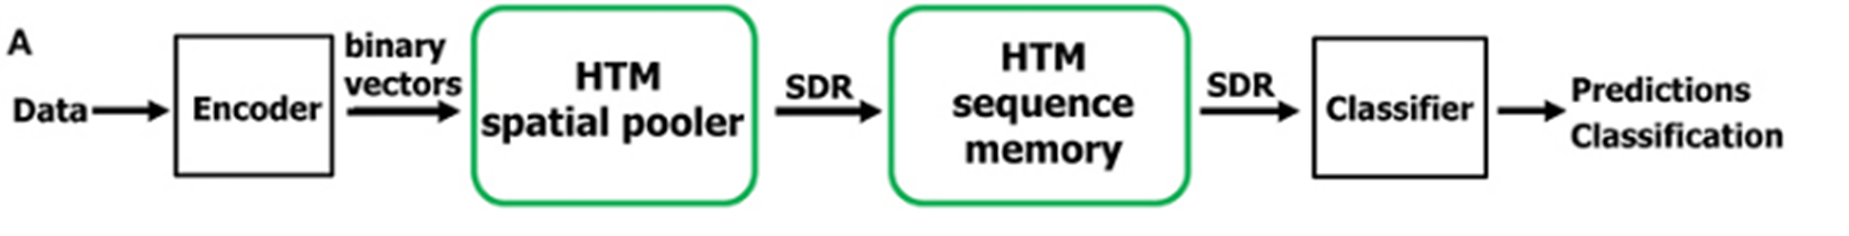
\includegraphics[scale=.40]{HtmPipeline.png}
\end{figure}

\subsection{Spatial Pooler}
Spatial Poolar is the second phase of HTM learning. It uses the output of the encoder to learn the SDR of the given input binary array. The idea for the spatial poolar SDR is to generate SDRs of the input which is the output of the encoder. Once the input SDR are learned, if the same input is given again, it tries to match already learned SDRs and then generates a similar matching SDR.In this method, it will disgunish, is it a same input which is already memorized or a different one.   



 








Explanation of how SDR datasets are handled and utilized.
Description of methods for loading SDR data from files.
Discussion of data structures and formats used for SDR datasets.

\section{Unit Testing and Exception Handling}
Overview of unit testing methodologies used.
Description of UnitTest1 class and its purpose.
Explanation of how test datasets are generated and utilized for testing.
Discussion of exception handling strategies implemented.
Explanation of how errors and exceptions are handled during file reading and data parsing.

\subsection{Applications of k-NN in machine learning}
KNN Algorithm is utilized in different applications across different sectors, mostly in classification. The common cases includes:


\subsubsection{Pattern Recognition}
KNN is used for the identification of specific patterns, it can be in a text. Like it predict the missing fill in the blanks. This also help in solving cache which are basically handwritten numbers. So, KNN can also
to identify these patterns.


\subsubsection{Healthcare}
The common use of KNN is health department is prediction of chances of cancer as well as heart attacks risks. The algorithm try to learn from most likely gene expressions. 

\subsubsection{Recommendation Engines}
When we surf on internet, the KNN algorithm can be used by the website to recommend us other additional content. This recommendation is based on user behaviour. But for larger datasets this approach is not optimal. 

\subsubsection{Data preprocessing}
Mostly we have a missing values in our dataset, KNN algorithm can help to determine those values. Those estimated missing values are also known as missing data imputation. 

\subsubsection{Finance}
The banks uses the credit card spending to predict the risk associated with the specific individual loan. As well as knn is used to determine the credit card worthiness of a loan application. So, KNN is used in variety of economic and finance departments. As well as the other common use case is currency exchange forecasting, stock market as well as trading futures etc.  





% conference papers do not normally have an appendix


% use section* for acknowledgment
\section*{Acknowledgment}


The authors would like to thank...





% trigger a \newpage just before the given reference
% number - used to balance the columns on the last page
% adjust value as needed - may need to be readjusted if
% the document is modified later
%\IEEEtriggeratref{8}
% The "triggered" command can be changed if desired:
%\IEEEtriggercmd{\enlargethispage{-5in}}

% references section

% can use a bibliography generated by BibTeX as a .bbl file
% BibTeX documentation can be easily obtained at:
% http://mirror.ctan.org/biblio/bibtex/contrib/doc/
% The IEEEtran BibTeX style support page is at:
% http://www.michaelshell.org/tex/ieeetran/bibtex/
%\bibliographystyle{IEEEtran}
% argument is your BibTeX string definitions and bibliography database(s)
%\bibliography{IEEEabrv,../bib/paper}
%
% <OR> manually copy in the resultant .bbl file
% set second argument of \begin to the number of references
% (used to reserve space for the reference number labels box)
\begin{thebibliography}{1}

\bibitem{1}
Cover, T., \& Hart, P. (1967). Nearest neighbor pattern classification. IEEE transactions on information theory, 13(1), 21-27.

\bibitem{2}
Cover, T., \& Hart, P. (1967). Nearest neighbor pattern classification. IEEE transactions on information theory, 13(1), 21-27.


\end{thebibliography}




% that's all folks
\end{document}


